\documentclass{beamer}

\usetheme{zg}

\title{Gradle}
\date{\today}
\author{Fernando Camargo}
\institute{ZG Soluções}


\begin{document}
\maketitle

\section{Por que uma ferramenta de Build?}

\begin{frame}{Por que uma ferramenta de Build?}
 \begin{outline}
   \1<1-> Projeto independente de IDE
   \1<2-> Automatização de build
 \end{outline}
\end{frame}

\section{Ant, Maven e Gradle}

\subsection{Ant}

\begin{frame}{Apache Ant}
 \begin{outline}
   \1<1-> Primeira build tool para Java
   \1<2-> Extrema flexibilidade
   \1<3-> Não impõe convenções em projetos Java
 \end{outline}
\end{frame}

\begin{frame}[fragile]{Exemplo de Ant}
 \begin{minted}[fontsize=\tiny]{xml}
<project>

    <target name="clean">
        <delete dir="build"/>
    </target>

    <target name="compile">
        <mkdir dir="build/classes"/>
        <javac srcdir="src" destdir="build/classes"/>
    </target>

    <target name="jar">
        <mkdir dir="build/jar"/>
        <jar destfile="build/jar/HelloWorld.jar" basedir="build/classes">
            <manifest>
                <attribute name="Main-Class" value="oata.HelloWorld"/>
            </manifest>
        </jar>
    </target>

    <target name="run">
        <java jar="build/jar/HelloWorld.jar" fork="true"/>
    </target>

</project>
  \end{minted}
\end{frame}

\begin{frame}{Problemas do Ant}
 \begin{outline}
   \1<1-> Flexível demais $\rightarrow$ projetos não possuem estrutura padrão
   \1<2-> Muito verboso $\rightarrow$ escreve-se muito para uma build simples
   \1<3-> Não possui gerenciamento de dependências
 \end{outline}
\end{frame}

\subsection{Maven}

\begin{frame}{Apache Maven}
 \begin{outline}
   \1<1-> Convenção sobre Configuração $\rightarrow$ escreve-se pouco para uma build simples
   \1<2-> Gerenciamento de dependências com resolução de dependências transitivas
 \end{outline}
\end{frame}

\begin{frame}{Estrutura de diretórios}
 \begin{table}[]
    \begin{tabular}{@{}ll@{}}
      \toprule
      Diretório           & Função                            \\ \midrule
      src/main/java       & Código fonte                      \\
      src/main/resources  & Recursos não compilados           \\
      src/test/java       & Código de testes                  \\
      src/test/resources  & Recursos não compilados de testes \\
      src/main/webapp     & Recursos WEB                      \\
      target              & Resultados de build               \\ \bottomrule
    \end{tabular}
  \end{table}
\end{frame}

\begin{frame}[fragile]{Exemplo de POM}
 \begin{minted}[fontsize=\tiny]{xml}
<project xmlns="http://maven.apache.org/POM/4.0.0" xmlns:xsi="http://www.w3.org/2001/XMLSchema-instance"
  xsi:schemaLocation="http://maven.apache.org/POM/4.0.0 http://maven.apache.org/xsd/maven-4.0.0.xsd">
  <modelVersion>4.0.0</modelVersion>
 
  <groupId>com.mycompany.app</groupId>
  <artifactId>my-app</artifactId>
  <version>1.0-SNAPSHOT</version>
  <packaging>jar</packaging>
 
  <name>Maven Quick Start Archetype</name>
  <url>http://maven.apache.org</url>
 
  <dependencies>
    <dependency>
      <groupId>junit</groupId>
      <artifactId>junit</artifactId>
      <version>4.8.2</version>
      <scope>test</scope>
    </dependency>
  </dependencies>
</project>
  \end{minted}
\end{frame}

\begin{frame}{Repositórios Maven}
  \begin{center}
    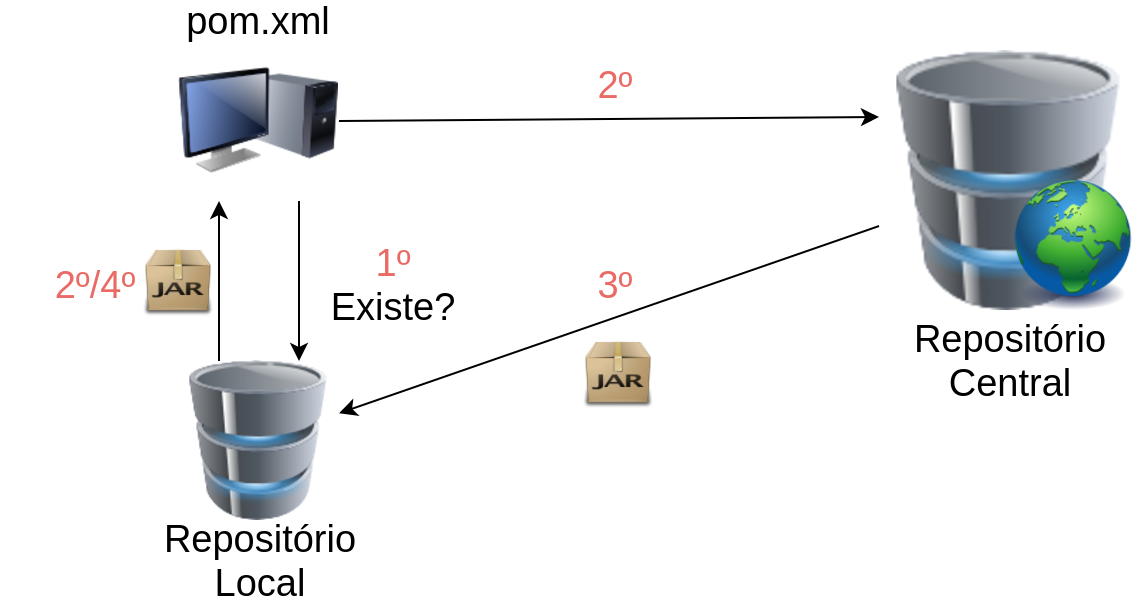
\includegraphics[width=0.9\textwidth]{repositorios-maven}
  \end{center}
\end{frame}

\begin{frame}{Problemas do Maven}
 \begin{outline}
   \1<1-> Rígido demais
   \1<2-> Uso de XML na configuração
   \1<3-> Ótimo para 90\% dos casos, complicado nos 10\% mais específicos
 \end{outline}
\end{frame}

\section{Gradle}

\begin{frame}{Por que Gradle?}
 \begin{outline}
   \1<1-> Combina as partes boas de Ant e Maven
    \2 Poder e Flexibilidade do Ant
    \2 Ciclo de vida e facilidade de uso do Maven
   \1<2-> Adiciona uma DSL e outras melhorias
 \end{outline}
\end{frame}

\begin{frame}{Características do Gradle}
 \begin{outline}
   \1<1-> Flexibilidade
   \1<2-> Completo controle
   \1<3-> Encadeamento de tarefas
   \1<4-> Gerenciamento de dependências
   \1<5-> Convenção sobre configuração
   \1<6-> Projetos multimódulo
   \1<7-> Extensível via plugins
   \1<8-> Groovy DSL
 \end{outline}
\end{frame}

\begin{frame}[fragile]{Exemplo de build.gradle}
 \begin{minted}[fontsize=\tiny]{groovy}
apply plugin: 'java'
 
version = '1.0'
 
repositories {
    mavenCentral()
}
 
dependencies {
    testCompile group: 'junit', name: 'junit', version: '4.11'
}
  \end{minted}
\end{frame}

\subsection{Script Gradle}

\begin{frame}{DSL = Domain Specific Language}
 \begin{outline}
   \1<1-> Pequena linguagem para solução de problemas específicos
  \0\visible<2->{Exemplo (SQL): \mintinline{sql}{SELECT * FROM Produtos WHERE ID = 5;}}
 \end{outline}
\end{frame}

\begin{frame}{Conceitos do Gradle}
 \begin{outline}
   \1<1-> Scripts Gradle são \alert{scripts de configuração}
    \2<2-> Execução do script $\rightarrow$ configuração de um \alert{objeto}
      \3<3-> Build script $\rightarrow$ \alert{Project}
      \3<4-> Init script $\rightarrow$ \alert{Gradle}
      \3<5-> Settings script $\rightarrow$ \alert{Settings}
    \2<6-> Propriedades e métodos do \alert{objeto} estão disponíveis no script
    \2<7-> Propriedades e métodos da interface \alert{Script} também disponíveis
 \end{outline}
\end{frame}

\begin{frame}{Build Script}
 \begin{outline}
   \1<1-> Composto \alert{instruções} e \alert{blocos} de script
   \1<2-> \alert{Instruções}
    \2 Invocação de métodos
    \2 Atribuição de propriedades
    \2 Definição de variáveis locais
    \2 Definição de métodos e classes
    \2 \alert{Qualquer elemento de script Groovy}
   \1<3-> \alert{Blocos} $\rightarrow$ invocação de um método com uma \alert{closure de configuração} como parâmetro
 \end{outline}
\end{frame}

\begin{frame}{Blocos de Script de base}
 \begin{table}[]
  \begin{tabular}{@{}ll@{}}
    \toprule
    Bloco                   & O que \alert{configura}                            \\ \midrule
    repositories \{ \}      & Os repositórios de dependências deste projeto      \\ \pause
    dependencies \{ \}      & As dependências deste projeto                      \\ \pause
    configurations \{ \}    & As configurações de dependências deste projeto     \\ \pause
    sourceSets \{ \}        & Os grupos de código e recursos deste projeto       \\ \pause
    artifacts \{ \}         & Os artefatos publicados deste projeto              \\ \pause
    buildscript \{ \}       & O classpath do build script deste projeto          \\ \pause
    allprojects \{ \}       & Este projeto e cada um dos sub projetos            \\ \pause
    subprojects \{ \}       & Apenas os sub projetos deste projeto               \\ \bottomrule
  \end{tabular}
\end{table}
\end{frame}

\subsection{Projetos e Tarefas}

\begin{frame}{Principais Tipos de Objetos}
 \begin{outline}
   \1<1-> Project
    \2<1-> Objeto alvo da configuração da build
    \2<2-> Através dele, pode-se acessar todas funcionalidades do Gradle
   \1<3-> Task
    \2<3-> Unidade atômica de trabalho da build
    \2<4-> Entidade central à lógica do Gradle
    \2<5-> Exemplos: compilar classes, gerar javadoc, etc.
   \1<6-> Script
    \2<7-> Interface com métodos específicos do Gradle
    \2<8-> Implementado por todos scripts
    \2<9-> Automaticamente implementado pelo build.gradle
 \end{outline}
\end{frame}

\begin{frame}[fragile]{Exemplo de Task e sua invocação}
 build.gradle:
 \begin{minted}[fontsize=\tiny]{groovy}
task hello {
  println "Hello world!"
}
 \end{minted}
 Invocação no terminal:
 \begin{minted}[fontsize=\tiny]{bash}
> gradle hello
 \end{minted}
\end{frame}

\begin{frame}[fragile]{Tasks padrões e dependências entre tasks}
 build.gradle:
 \begin{minted}[fontsize=\tiny]{groovy}
defaultTasks 'clean', 'compile'

task clean << {
  println "Executando clean"
}

task compile << {
  println "Executando compile"
}

task other(dependsOn: 'compile') << {
  println "Executando other"
}
 \end{minted}
 Invocação no terminal:
 \begin{minted}[fontsize=\tiny]{bash}
> gradle
Executando clean
Executando compile
> gradle other
Executando compile
Executando other
 \end{minted}
\end{frame}

\subsection{Plugins}

\begin{frame}{Voltamos ao Ant?}
 \begin{outline}
   \1<1-> Gradle suporta plugins, como o Maven
   \1<2-> Esses plugins registram Tasks e SourceSets
   \1<3-> Convenção sobre Configuração $\rightarrow$ mesma estrutura de diretórios do Maven
 \end{outline}
\end{frame}

\begin{frame}[fragile]{Exemplos de plugins}
 \begin{minted}[fontsize=\tiny]{groovy}
buildscript {
  dependencies {
    classpath 'com.android.tools.build:gradle:2.3.2'
  }
}
 
apply plugin: 'java'
apply plugin: 'groovy'
apply plugin: 'com.android.application'
 \end{minted}
\end{frame}

\subsection{Gerenciamento de dependências}

\begin{frame}{Gerenciamento de dependências}
 \begin{outline}
   \1<1-> Compatível com Maven e Ivy
     \2 Suporta repositórios Maven
   \1<2-> Gerenciamento de dependências transitivas
   \1<3-> Dependências/projetos são identificados por \mintinline{groovy}{"groupId:artifactId:version"}
 \end{outline}
\end{frame}

\begin{frame}{Definindo groupId, artifactId e version}
 \begin{outline}
   \1<1-> As propriedades \alert{group} e \alert{version} podem ser definidas em \textbf{gradle.build} ou \textbf{gradle.properties}
    \2<2-> build.gradle:
     \3\visible<2->{\mintinline{groovy}{group = "br.com.zeroglosa"}\\\mintinline{groovy}{version = "1.0.0"}}
    \2<3-> gradle.properties:
     \3\visible<3->{group=br.com.zeroglosa\\version=1.0.0}
   \1<4-> A propriedade \alert{name} pode ser definida em settings.gradle:
    \2\visible<4->{\mintinline{groovy}{rootProject.name = "artifactId"}}
    \2<5-> Se não definida, considera-se o nome da pasta do projeto
 \end{outline}
\end{frame}

\begin{frame}[fragile]{Exemplos de dependências}
 \begin{minted}[fontsize=\tiny]{groovy}
apply plugin: 'java'

repositories {
  mavenCentral()
  mavenLocal()
  jcenter()
}

dependencies {
  compile 'com.google.guava:guava:20.0'
  
  testCompile 'junit:junit:4.12'
}
 \end{minted}
\end{frame}


\begin{frame}{Gerenciamento de dependências transitivas}
 \begin{outline}
   \1<1-> Dependências podem possuir dependências transitivas
    \2<2-> Que podem possuir outras dependências transitivas
   \1<3-> Diferentes versões podem ser especificadas
    \2 \textbf{A:1.0} $\rightarrow$ \textbf{B:1.2}
    \2 \textbf{C:1.5} $\rightarrow$ \textbf{B:1.3}
    \2 \textbf{D:2.1} $\rightarrow$ \textbf{C:1.6} $\rightarrow$ \textbf{B:1.5}
    \2<4-> Qual versão de \textbf{A}, \textbf{B}, \textbf{C} e \textbf{D}?
 \end{outline}
\end{frame}

\begin{frame}{Gerenciamento de dependências transitivas}
 \begin{outline}
   \1<1-> Regras para definição de versões:
    \2<1-> Primeiro mais pŕoximo
      \3 Dependência de nível mais alto tem prioridade
      \3 Dependência direta tem prioridade sobre transitiva
    \2<2-> Primeiro encontrado (desempate)
      \3 Primeira encontrada é usada
   \1<3-> Problema:
    \2 \textbf{A:1.0} $\rightarrow$ \textbf{B:1.2}
    \2 \textbf{C:1.5} $\rightarrow$ \textbf{B:1.3}
    \2 \textbf{D:2.1} $\rightarrow$ \textbf{C:1.6} $\rightarrow$ \textbf{B:1.5}
   \1<4-> Solução:
    \2 A:1.0
    \2 B:1.2
    \2 C:1.5
    \2 D:2.1
 \end{outline}
\end{frame}

\begin{frame}[fragile]{Exclusão de dependências}
 \begin{minted}[fontsize=\tiny]{groovy}
apply plugin: 'java'

repositories {
  mavenCentral()
  mavenLocal()
  jcenter()
}

dependencies {
  compile('org.hibernate:hibernate-core:5.2.10.Final'){
    exclude module: 'dom4j'
    exclude group: 'org.javassist', module: 'javassist'
  }
  
  testCompile 'junit:junit:4.12'
}
 \end{minted}
\end{frame}

\section{Java Plugin}

\begin{frame}{Tasks}
  \begin{center}
    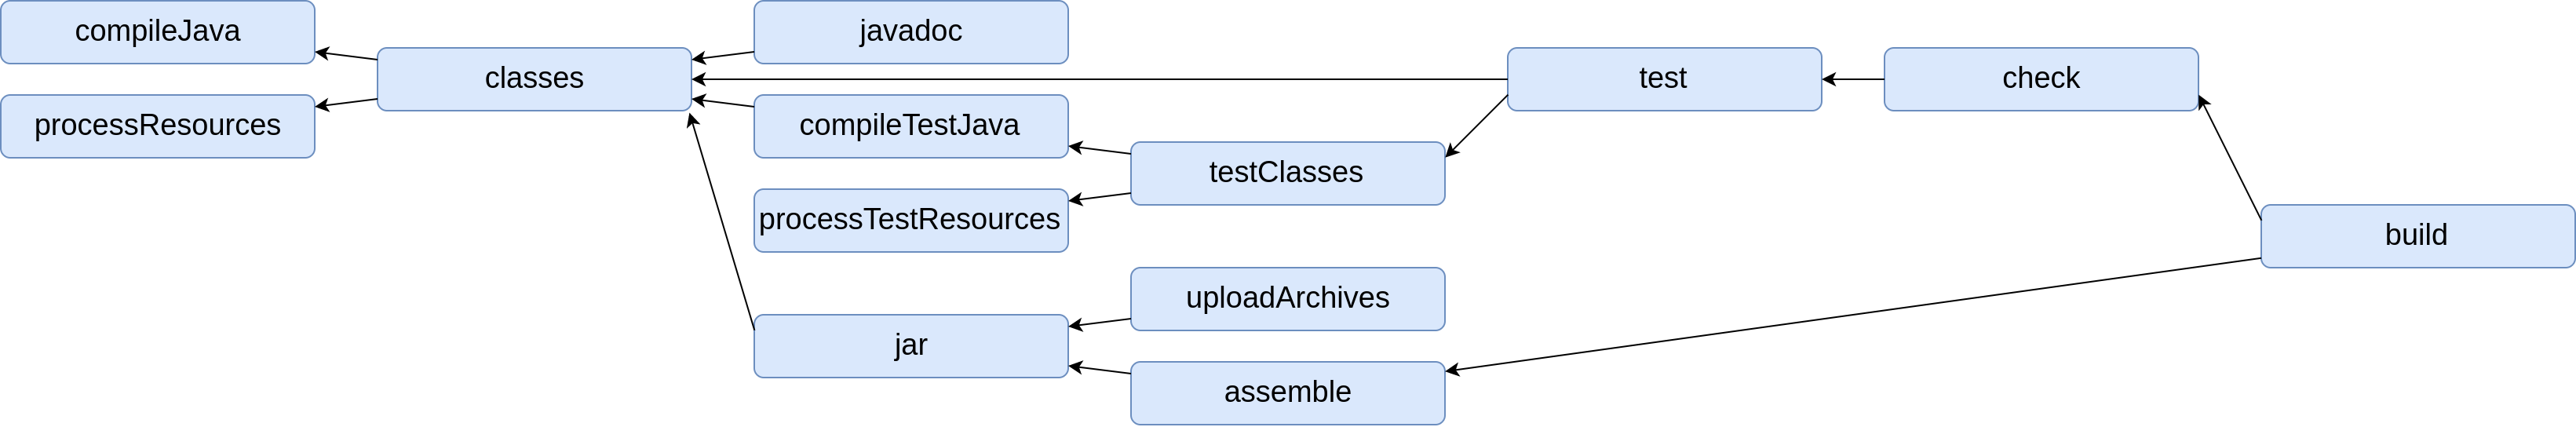
\includegraphics[width=\textwidth]{java-plugin-tasks}
  \end{center}
\end{frame}


\begin{frame}{Estrutura do projeto}
 \begin{table}[]
    \begin{tabular}{@{}ll@{}}
      \toprule
      Diretório                        & Função                              \\ \midrule
      src/main/java                    & Código fonte de produção            \\
      src/main/resources               & Recursos de produção                \\
      src/test/java                    & Código de testes                    \\
      src/test/resources               & Recursos de testes                  \\
      src/\alert{sourceSet}/java       & Código de dado \alert{dataSource}   \\
      src/\alert{sourceSet}/resources  & Recursos de dado \alert{dataSource} \\ \bottomrule
    \end{tabular}
  \end{table}
\end{frame}

\begin{frame}{Configurações de dependências/Escopos}
  \begin{center}
    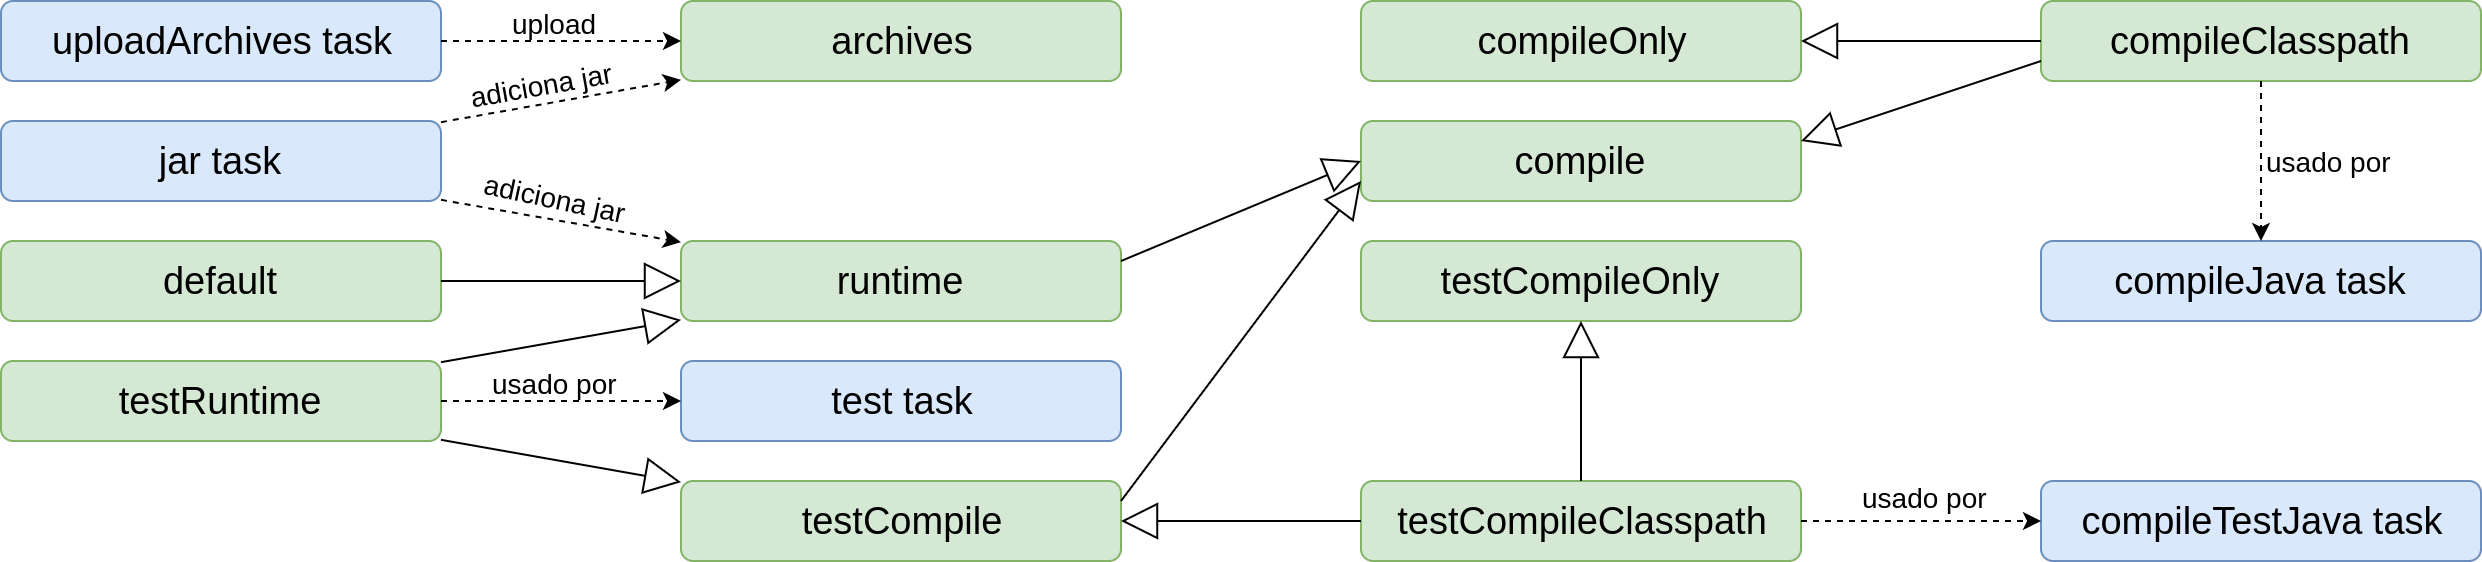
\includegraphics[width=\textwidth]{java-plugin-dependencies}
  \end{center}
\end{frame}

\section{Conclusões}

\begin{frame}{Conclusões}
 \begin{outline}
   \1<1-> Existem \alert{muitos plugins}, inclusive para diversas linguagens
   \1<2-> Grande \alert{flexibilidade}, inclusive para desenvolver plugins
   \1<3-> Permite fácil \alert{automatização} da build
   \1<4-> \alert{Convenção} sobre configuração
   \1<5-> \alert{DSL} compacta e poderosa
 \end{outline}
\end{frame}

\end{document}